\section{Controller Setup}
\label{chap:Controller}
% Talk about definition and setup of the controller in MATLAB, describing all the parameters set, then talk about the simulink model and then talk about the "partitioning" of functionalities for the tests (Path following - Static avoidance- Dynamic avoidance)
% In this section we will describe in detail how we implemented the controller in the MATLAB/Simulink environment.
% 1) Implementazione  MPC in Matlab
% 2) Implementazione MPC in Simulink
% 3) Partitioning delle funzionalità del MPC

% 1) Together Copy and paste from misc.tex MATLAB implementation


Matlab's Model Predictive Control Toolbox provides functions, an app, and Simulink blocks for designing and simulating controllers using linear and nonlinear model predictive control (MPC) \cite{MPCToolbox}. Thanks to the toolbox we specified the plant model, horizons, constraints, and weights. By running closed-loop simulations, we evaluated controller performance and adjusted its behavior by varying weights and constraints at run time.

\subsection{MPC Initialisation}
Initialisation phase requires the definition of all the parameters needed for the execution of the controller.
First of all we have created a MPC object passing as input the discretized state-space model of the plant, the prediction horizon and the control horizon.
\\Assuming that the car is already traveling at a speed \textit{V}, the initial conditions for the other states is set taking the first point in the reference path, and for the two inputs it is set equal to zero. Exploiting the function \textit{odometer} we computed the total distance covered by the car following the scenario in order to let the simulation terminates exactly when the road ends.
\\Subsequently we defined the constraints on inputs (Table \ref{tab:steering} and \ref{tab:throttle}) and the weights for the cost function, which correctly tuned, guarantee that the vehicle follows the reference without going off the road  i.e. stays within the lane width limits and is capable to avoid an obstacle when is inside the sensors detection range.



\subsection{MPC Algorithm}  
Once the controller has been initialised, all is ready to let the simulation begin.
\\At each time$-$step, different instructions are repeated in a \textit{for} loop to simulate the controller in a closed$-$loop fashion. Figure \ref{fig:MPC_scheme} graphically shows the general concept behind a model predictive control; below it's described the Matlab algorithm that follows the same scheme.
\begin{figure}[H]
    \centering
    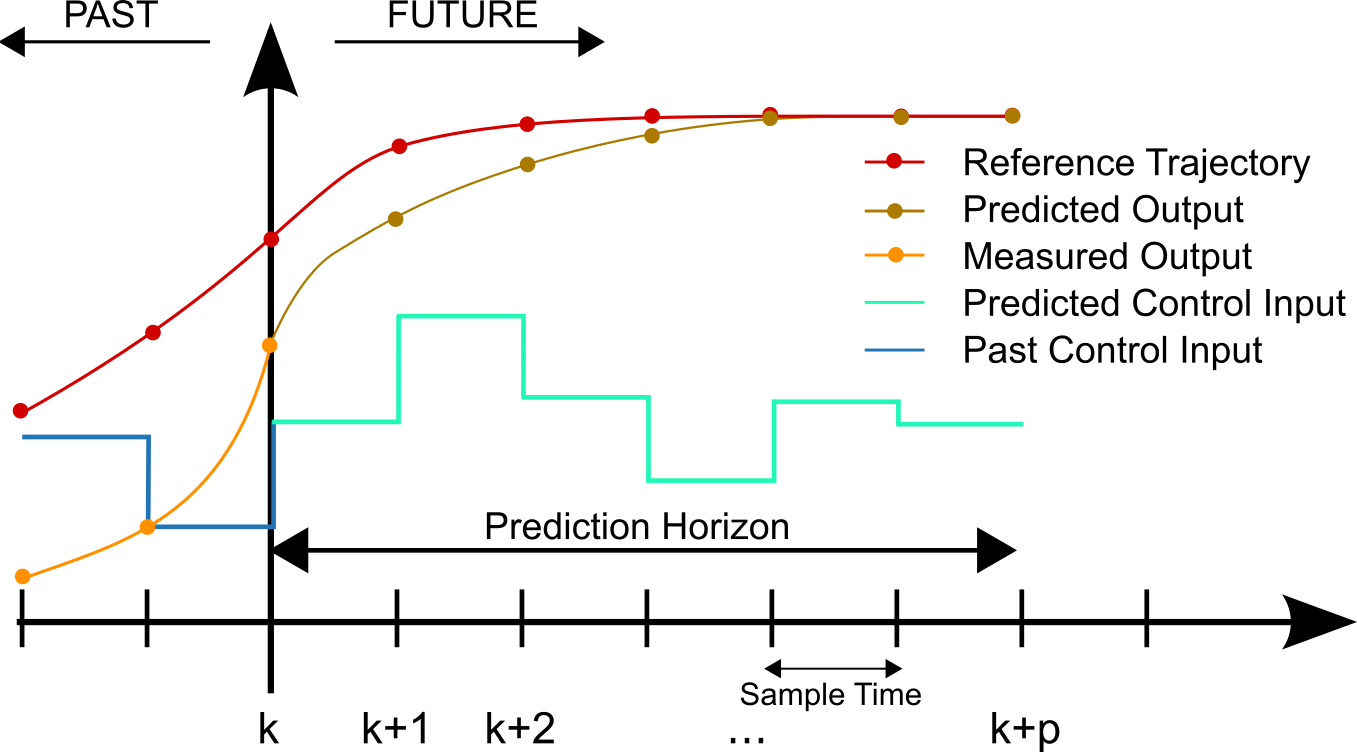
\includegraphics[width=0.9\textwidth]{Figures/MPC_scheme_basic.png}
    \caption{MPC algorithm scheme}
    \label{fig:MPC_scheme}
\end{figure}
First, the current state and the inputs are used in the function \textit{obstacleVehicleModelDT} to generate a discrete$-$time model, using the Zero$-$Order Hold (ZOH) method, and consequently to generate the nominal conditions for the discrete plant and the measurements. Then, the reference path is updated: starting from an index that is increased at each cycle, the trajectory data are read along the prediction horizon length. Once the new plant model and nominal conditions are calculated, they are used as inputs for the \textit{mpcmoveAdaptive} Matlab command that computes the Adaptive MPC control action at current time. This same control action is subsequently used as input to the \textit{VehicleModelCT\_DYN\_ode} function that outputs the differential equations relative to the vehicle dynamic model; these equations are integrated from 0 to the time$-$step using the \textit{ode45} function.
\\In the end, the loop is concluded assigning to the next state\footnote{The \textit{next} state in the current cycle will correspond to the \textit{current} state in the successive cycle as the index is increased} the result of the integration.\\
The pattern described above is repeated \textit{n} times, where \textit{n} represent the ratio between the set simulation duration and resolution.



% 2) Alessandro  SIMULINK
\subsection{Simulink Model}

In order to run closed-loop simulations a Simulink model has been designed because of the availability of many useful tools to test and validate the model. For the sake of clarity in reading and debugging the whole system, some of the Simulink blocks have been grouped in subsystems and a mask applied to some of them. 
% IMMMAGINE DA CAMBIARE QUANDO SIMULINK SARA' FINITO
\begin{figure}[H]
    \centering
    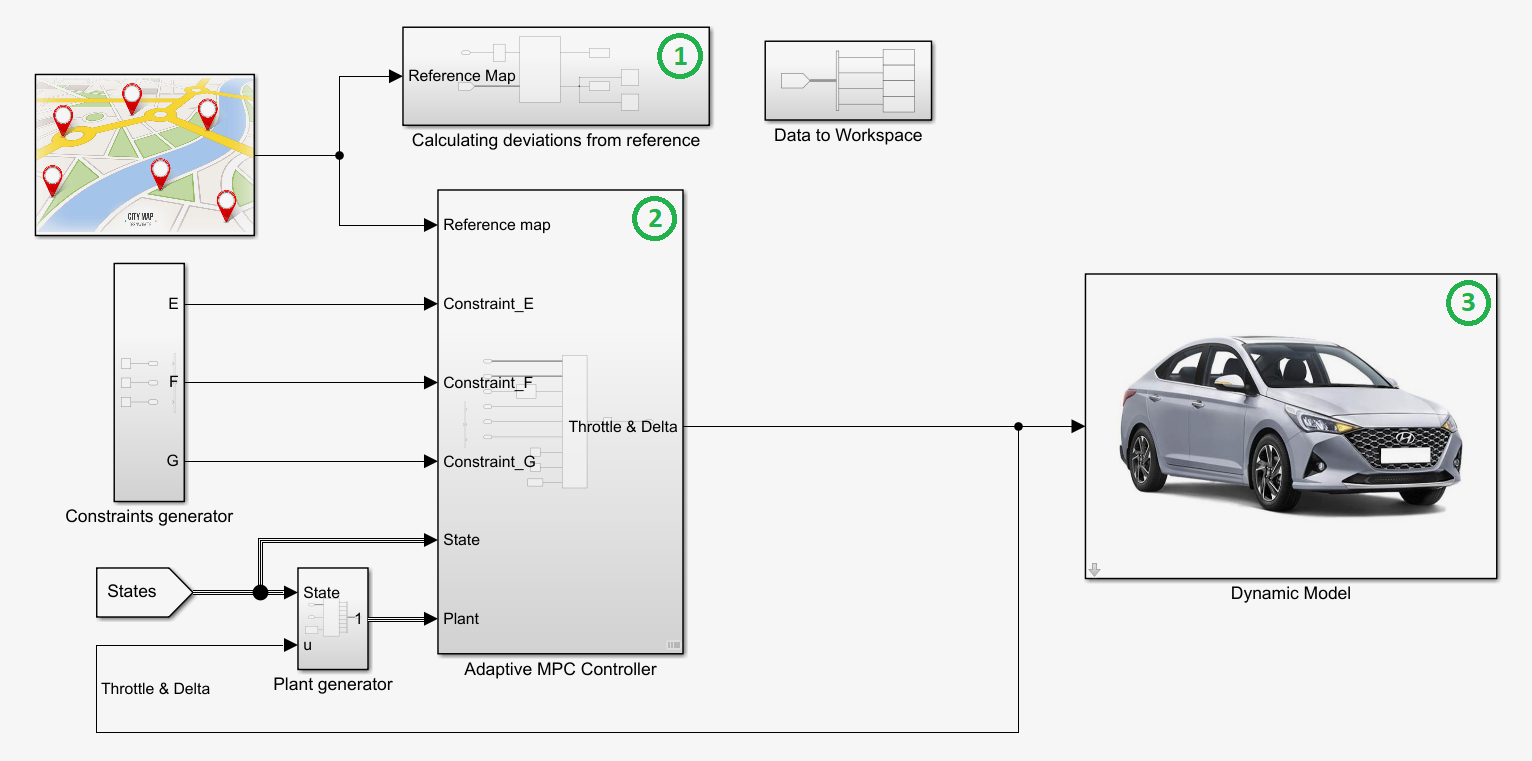
\includegraphics[width=\textwidth]{Figures/simulink_main_mod.png}
    \caption{Simulink main}
    \label{fig:simulink_main_mod}
\end{figure} 
In Figure \ref{fig:simulink_main_mod} the main system is depicted: the process simulated by these blocks is coherent with the MPC algorithm described in the previous section and the the numbers in green enumerate the three major subsystems and will be analyzed in the following.
\begin{figure}[H]
    \centering
    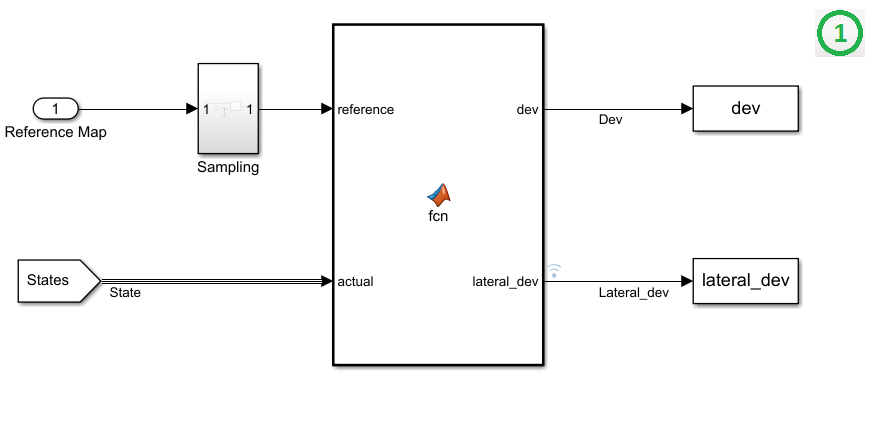
\includegraphics[width=0.9\textwidth]{Figures/simulink_deviations_mod.png}
    \caption{Simulink subsystem to calculate deviations}
    \label{fig:simulink_deviations_mod}
\end{figure}
Namely, the content of the subsystem numbered 1 is displayed in Figure \ref{fig:simulink_deviations_mod}: the main purpose of these blocks is calculating a deviation from the reference in order to test controller and will be analyzed in details in the next Chapter \ref{chap:path_following}; in order to pass the proper number of reference way-points, a sampling subsystem is used as a input to the Matlab function block. A similar sampling subsystem is used also as input to the reference of the simulink block \textit{Adaptive MPC}: in Figure \ref{fig:simulink_mpc_mod} below indeed, are showed the blocks composing the subsystem \textit{Adaptive MPC Controller} and in the blue rectangle is enlighted how the content of the reference map is sampled\footnote{ The sampling subsystems displayed in Fig.\ref{fig:simulink_deviations_mod} and Fig.\ref{fig:simulink_mpc_mod} are both structured in the same way (selector and counter basically) but are different in the sampling rate}.
\begin{figure}[H]
    \centering
    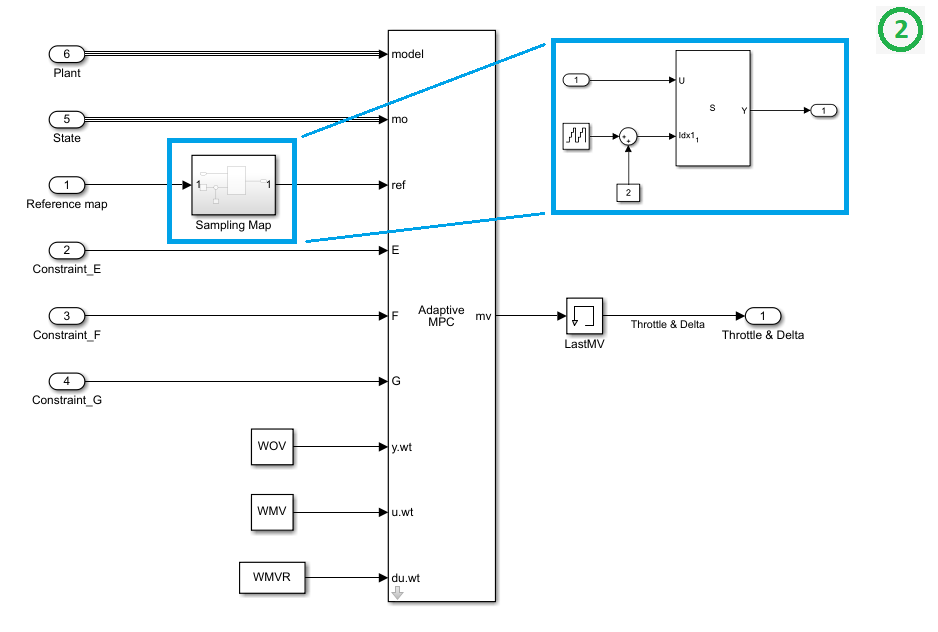
\includegraphics[width=0.9\textwidth]{Figures/simulink_mpc_mod.png}
    \caption{Simulink subsystem: Adaptive MPC controller}
    \label{fig:simulink_mpc_mod}
\end{figure}
The subsystem \textit{Dynamic Model} displayed in Fig.\ref{fig:simulink_main_mod} has as a mask the picture of an Hyundai Verna as this is the vehicle whose parameters are used in the simulation. Also for these blocks $-$ Fig.\ref{fig:simulink_dyn_mod_mod}, the main purpose is calling an already designed Matlab function that in this case is the \textit{VehicleModelCT\_DYN} one, previously described in Chap.\ref{chap:Vehicle_model}.
\begin{figure}[H]
    \centering
    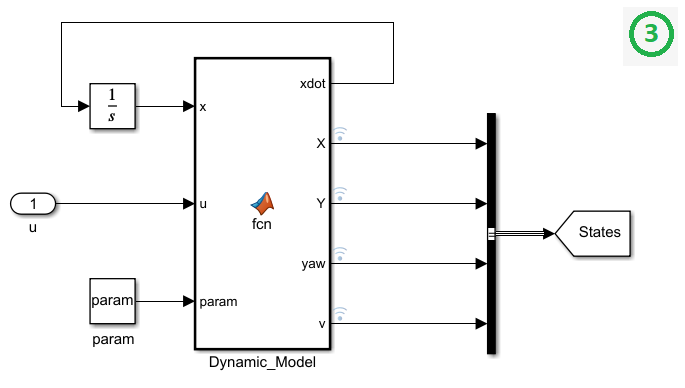
\includegraphics[width=0.9\textwidth]{Figures/simulink_dyn_mod_mod.png}
    \caption{Simulink subsystem: Dynamic Model}
    \label{fig:simulink_dyn_mod_mod}
\end{figure} 





% 3) Gianvincenzo   Partitioning of functionalities
\subsection{Partitioning of the MPC functionalities}
The developed MPC controller is supposed to carry out three main tasks: 
\begin{itemize}
    \item \textbf{Path following}: the car must be able to follow a given reference path without exceeding a predetermined threshold distance;
    \item \textbf{Static obstacle avoidance}: the car must sense and dodge any kind of stationary obstacle present on the road i.e. road construction sites, holes, trees,  car accident, etc.;
    \item \textbf{Dynamic obstacle avoidance}: the car has the ability to perform overtaking maneuvers in the event that other moving vehicles, cyclists, pedestrians or animals are present in the same lane. The avoidance maneuver must be accomplished whether they are traveling in the same direction as the vehicle or in the opposite one.
\end{itemize}
Figure \ref{fig:dynamic_avoidance} shows how the ego-car (red) performs the overtaking maneuver: firstly it analyze the surrounding thanks to the on-board sensors and if it has enough space to achieve the lane change accordingly to the position and speed of the two moving obstacle (white cars) it plans the trajectory to follow to achieve the avoidance (blue path). Once the ego-car has planned a feasible path it starts to steer and accelerate arriving to the middle lane overtaking the car in the rightmost lane.

\begin{figure}[H]
    \centering
    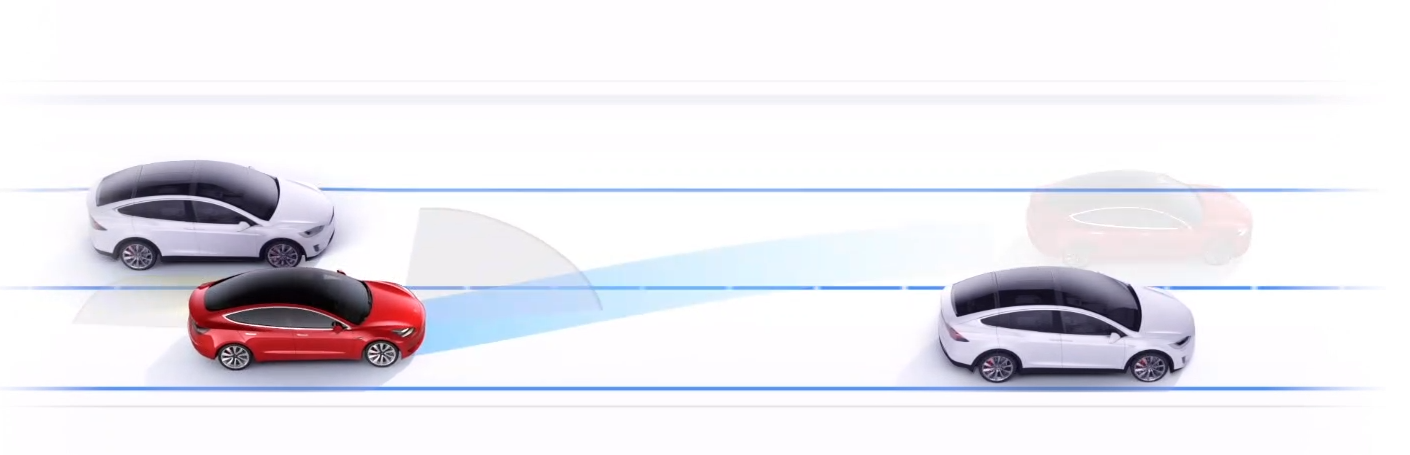
\includegraphics[width=1\textwidth]{Figures/dynamic_avoidance.png}
    \caption{Dynamic obstacle avoidance maneuver on a three lanes road}
      \label{fig:dynamic_avoidance}
\end{figure}
In order to perform the path following task the MPC collects at each timestep the successive waypoints of the map for the duration of the prediction horizon and elaborates an optimal trajectory and control action to minimize the a cost function of the controller.
\\Things get harder when obstacles are present on the road, either they are static or moving: we assumed to know ``a priori" the position of the static obstacle or the trajectory that the moving obstacle is following, in such way thanks to the MATLAB function \textit{``detectionFun"} we augmented the algorithm used for the path following with the capability to detect obstacles within the sensing range of the vehicle, thus allowing to promptly start and execute the avoidance maneuver always being outside the so called \textit{``safe zone"} of the obstacle.\\ Figure \ref{fig:static_avoidance_example} plots an example scenario for static obstacle avoidance, where: 
\begin{itemize}
    \item the \textbf{ego car} is represented by the green dot with the black boundary;
    \item the \textbf{horizontal lanes} are represented by the dashed blue lines;
    \item the \textbf{static obstacle} is represented by the red x with the black boundary;
    \item the \textbf{safe zone} is highlighted by the dashed red boundary.
\end{itemize} 

\begin{figure}[H]
    \centering
    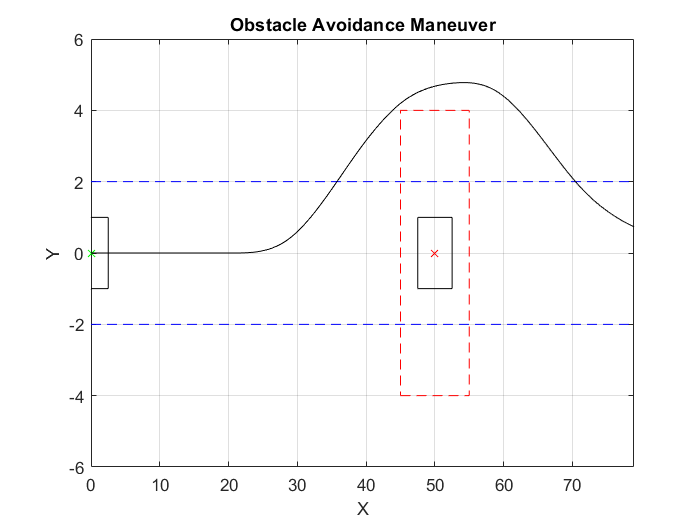
\includegraphics[width=1\textwidth]{Figures/static_avoidance_example.png}
    \caption{Example of static obstacle avoidance maneuver}
      \label{fig:static_avoidance_example}
\end{figure} 
